%!TeX options = -shell-escape
\documentclass{article}
\usepackage{tikz}
\usetikzlibrary{external}
\tikzexternalize
\begin{document}
\begin{center}
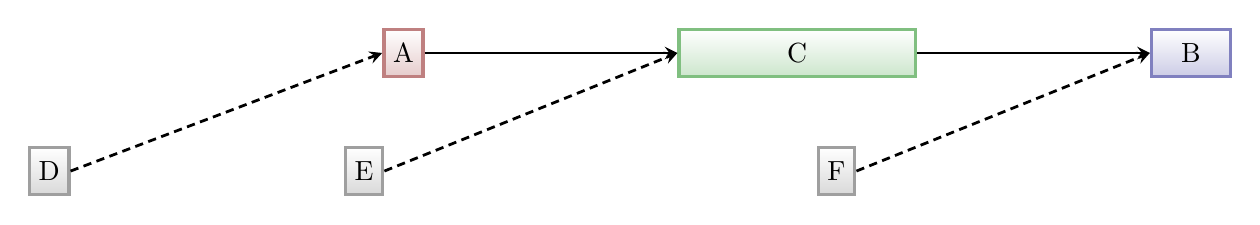
\begin{tikzpicture}
[
basic/.style={
% The shape:
rectangle,
% The size:
minimum height=6mm,
% The border:
very thick,
draw=red!50!black!50, % 50% red and 50% black,
% and that mixed with 50% white
% The filling:
top color=white, % a shading that is white at the top...
bottom color=red!50!black!20, % and something else at the bottom
},
proof/.style={
% The shape:
rectangle,
% The size:
minimum height=6mm,
% The border:
very thick,
draw=gray!50!black!50, % 50% red and 50% black,
% and that mixed with 50% white
% The filling:
top color=white, % a shading that is white at the top...
bottom color=gray!50!black!20, % and something else at the bottom
},
adapter/.style={
% The shape:
rectangle,
% The size:
minimum width=3cm,
minimum height=6mm,
% The border:
very thick,
draw=green!50!black!50, % 50% red and 50% black,
% and that mixed with 50% white
% The filling:
top color=white, % a shading that is white at the top...
bottom color=green!50!black!20, % and something else at the bottom
},
decorator/.style={
% The shape:
rectangle,
% The size:
minimum width=1cm,
minimum height=6mm,
% The border:
very thick,
draw=blue!50!black!50, % 50% red and 50% black,
% and that mixed with 50% white
% The filling:
top color=white, % a shading that is white at the top...
bottom color=blue!50!black!20, % and something else at the bottom
}
]
    \node[below, align=justify, basic] (a) at (2.5, 0) {A};
    \node[below, align=justify, decorator] (c) at (12.5, 0) {B};
    \node[below, align=justify, adapter] (b) at (7.5, 0) {C};
    \node[below, align=justify, proof] (d1) at (-2, -1.5) {D};
    \node[below, align=justify, proof] (d2) at (2, -1.5) {E};
    \node[below, align=justify, proof] (d3) at (8, -1.5) {F};
    \draw[-{stealth[black]}, line width=1pt] (a.east) -- (b.west);
    \draw[-{stealth[black]}, line width=1pt] (b.east) -- (c.west);
    \draw[-{stealth[black]}, line width=1pt, densely dashed] (d1.east) -- (a.west);
    \draw[-{stealth[black]}, line width=1pt, densely dashed] (d2.east) -- (b.west);
    \draw[-{stealth[black]}, line width=1pt, densely dashed] (d3.east) -- (c.west);
\end{tikzpicture}
\end{center}
\end{document}

